\documentclass[11pt,a4paper]{article}

% ---- Encodage et langue ----
\usepackage[utf8]{inputenc}
\usepackage[T1]{fontenc}
\usepackage[french]{babel}

% ---- Mise en page ----
\usepackage[a4paper,margin=2.5cm]{geometry}
\usepackage{setspace}
\onehalfspacing
\usepackage{parskip}

% ---- Figures et tableaux ----
\usepackage{graphicx}
\usepackage{float}
\usepackage{caption}
\usepackage{subcaption}
\usepackage{booktabs}
\usepackage{array}
\usepackage{amssymb}

% ---- Diagramme de Gantt ----
\usepackage{pgfgantt}
\usepackage{xcolor}

% ---- Liens et références ----
\usepackage[hidelinks]{hyperref}
\usepackage{url}

% ---- En-tête et pied de page ----
\usepackage{fancyhdr}
\pagestyle{fancy}
\fancyhf{}
\fancyhead[L]{Projet 805 — Zones blanches 4G}
\fancyhead[R]{2025--2026}
\fancyfoot[C]{\thepage}
\renewcommand{\headrulewidth}{0.4pt}

\begin{document}

% ============================================================
% ---- Page de garde ----
% ============================================================
\begin{titlepage}
\thispagestyle{empty}
\centering

\vspace*{0.5cm}
{\scshape\Large Université de Reims Champagne-Ardenne\par}
{\scshape\large Master 1 — Intelligence Artificielle\par}
\vspace{0.4cm}
{\large Info0805 — Gestion de projets\par}
\vspace{0.1cm}
{\large Info0806 — Projet de programmation 2\par}

\vfill

\rule{\linewidth}{1pt}\\[0.8cm]
{\huge\bfseries Cartographie des zones blanches 4G\\[0.4cm]
sur les grands axes routiers français\par}
\vspace{0.8cm}
{\Large\itshape Croisement géospatial des données ARCEP\\et OpenStreetMap\par}
\vspace{0.6cm}
\rule{\linewidth}{1pt}

\vfill

{\large
\begin{tabular}{c}
  \textbf{Thomas \textsc{Chevalier}} \\[0.3cm]
  \textbf{Ethan \textsc{Cocu}}
\end{tabular}\par}

\vspace{1.2cm}

{\large Sous l'encadrement de\\[0.2cm]
\textbf{Hacène \textsc{Fouchal}}\par}

\vfill

{\large Année universitaire 2025--2026\par}
\vspace{0.5cm}

\end{titlepage}

% ============================================================
% ---- Sommaire ----
% ============================================================
\thispagestyle{empty}
\tableofcontents
\newpage

% ============================================================
\section{Gestion de projet}
% ============================================================

\subsection{Présentation de l'équipe et des rôles}

Le projet a été réalisé en binôme dans le cadre des UE Info0806 (Projet de programmation 2) et Info0805 (Gestion de projets), sous l'encadrement du professeur Hacène Fouchal. La répartition des responsabilités suit une matrice RACI simplifiée :

\begin{table}[H]
  \centering
  \caption{Matrice RACI du projet.}
  \begin{tabular}{lccc}
    \toprule
    \textbf{Tâche} & \textbf{T. Chevalier} & \textbf{E. Cocu} & \textbf{H. Fouchal} \\
    \midrule
    Analyse des besoins et rédaction CDC  & R & R & A \\
    Collecte et préparation des données   & R & C & I \\
    Développement pipeline étape 1        & R & R & I \\
    Développement pipeline étape 2        & C & R & I \\
    Optimisation (overlay tuilé parallèle) & C & R & I \\
    Analyse territoriale et set cover     & R & C & I \\
    Analyse des résultats                 & R & R & A \\
    Rédaction du rapport                  & R & R & A \\
    \bottomrule
  \end{tabular}
\end{table}

Concrètement, la répartition du travail a été la suivante : \textbf{Thomas Chevalier} s'est chargé de la collecte des données, de l'étape~1 (fusion des couvertures) et de la rédaction du rapport ; \textbf{Ethan Cocu} a développé l'étape~2 (routes couvertes) et l'étape~3 (placement des antennes). L'analyse des besoins et les décisions structurantes ont été menées conjointement.

\subsection{Objectifs SMART}

Les objectifs du projet ont été formulés selon la méthode SMART :

\begin{itemize}
  \item \textbf{Spécifique} : cartographier les zones blanches 4G sur le réseau des grands axes routiers de la France métropolitaine, à partir des données open data ARCEP.
  \item \textbf{Mesurable} : calculer un taux de couverture par longueur cumulée de route, sur l'ensemble des autoroutes et axes principaux identifiés dans OpenStreetMap.
  \item \textbf{Acceptable} : les données ARCEP sont librement accessibles et les outils Python (GeoPandas, Shapely) sont maîtrisés par l'équipe.
  \item \textbf{Réaliste} : le projet est dimensionné pour un binôme étudiant sur un semestre, avec un encadrant disponible pour validation.
  \item \textbf{Temporellement défini} : livraison du rapport et du pipeline finalisé pour la fin du mois de mai 2026.
\end{itemize}

\subsection{Planification et jalons}

Le projet s'est déroulé sur le second semestre de l'année universitaire 2025--2026. Les séances de travail encadrées (Info0806-TP) ont servi de jalons réguliers pour faire le point sur l'avancement. Le tableau suivant présente le rétro-planning du projet :

\begin{table}[H]
  \centering
  \caption{Rétro-planning du projet.}
  \small
  \begin{tabular}{llll}
    \toprule
    \textbf{Phase} & \textbf{Période} & \textbf{Livrable / Jalon} & \textbf{Statut} \\
    \midrule
    \multicolumn{4}{l}{\textit{Projet initial — Modélisation de la couverture antenne 4G/5G}} \\[2pt]
    Analyse des besoins     & Janvier 2026         & Définition du périmètre initial          & \checkmark \\
    Cahier des charges      & Février 2026         & Mini CDC envoyé (18/02/2026)              & \checkmark \\
    \midrule
    \multicolumn{4}{l}{\textit{Réorientation du projet — Mars 2026}} \\[2pt]
    Changement de périmètre & Mars 2026            & Nouveau sujet défini par M.~Fouchal       & \checkmark \\
    \midrule
    \multicolumn{4}{l}{\textit{Projet final — Cartographie des zones blanches 4G}} \\[2pt]
    Collecte des données    & Mars 2026            & Données ARCEP/OSM/IGN récupérées          & \checkmark \\
    Développement étape 1   & Mars 2026            & Pipeline fusion opérateurs                & \checkmark \\
    Développement étape 2   & Mars -- Avril 2026   & Pipeline croisement routier               & \checkmark \\
    Optimisation            & Avril 2026           & Overlay tuilé multithreadé                & \checkmark \\
    Analyse territoriale    & Avril -- Mai 2026    & Stats dépt/région + set cover             & \checkmark \\
    Analyse et rédaction    & Mai 2026             & Rapport final                             & \checkmark \\
    Livraison               & Mai 2026             & Dépôt rapport + code                      & \checkmark \\
    \bottomrule
  \end{tabular}
\end{table}

La figure~\ref{fig:gantt} présente le diagramme de Gantt correspondant, faisant apparaître la rupture de mars.

\begin{figure}[H]
\centering
\resizebox{\textwidth}{!}{%
\begin{ganttchart}[
  hgrid,
  vgrid={*{1}{dotted}, *{1}{dotted}, black!60, *{1}{dotted}, *{1}{dotted}, black!60,
         *{1}{dotted}, *{1}{dotted}, black!60, *{1}{dotted}},
  x unit=1.6cm,
  y unit title=0.55cm,
  y unit chart=0.6cm,
  title height=1,
  bar height=0.5,
  bar label font=\small,
  title label font=\bfseries\footnotesize,
  group label font=\bfseries\small,
  group top shift=0.25,
  group height=0.25,
]{1}{10}
  \gantttitle{Janvier}{2} \gantttitle{Février}{2} \gantttitle{Mars}{2}
  \gantttitle{Avril}{2} \gantttitle{Mai}{2} \\
  %--- Projet initial
  \ganttgroup[group/.append style={fill=orange!50}]{Projet initial}{1}{4} \\
  \ganttbar[bar/.append style={fill=orange!40}]{Analyse des besoins}{1}{2} \\
  \ganttbar[bar/.append style={fill=orange!40}]{Rédaction CDC}{3}{4} \\
  \ganttmilestone[milestone/.append style={fill=orange!80}]{CDC (18/02)}{4} \\
  %--- Projet final
  \ganttgroup[group/.append style={fill=blue!40}]{Projet final}{5}{10} \\
  \ganttbar[bar/.append style={fill=blue!35}]{Collecte données ARCEP}{5}{6} \\
  \ganttbar[bar/.append style={fill=blue!35}]{Étape 1 — Fusion opérateurs}{5}{6} \\
  \ganttbar[bar/.append style={fill=blue!35}]{Étape 2 — Croisement routier}{6}{8} \\
  \ganttbar[bar/.append style={fill=blue!35}]{Optimisation (overlay tuilé)}{7}{8} \\
  \ganttbar[bar/.append style={fill=blue!35}]{Analyse territoriale}{8}{9} \\
  \ganttbar[bar/.append style={fill=blue!35}]{Rédaction rapport}{9}{10} \\
  \ganttmilestone[milestone/.append style={fill=blue!70}]{Livraison}{10} \\
  %--- Ligne de réorientation
  \ganttvrule[vrule/.append style={draw=red!80, dashed, line width=1.5pt}]{Réorientation}{4.5}
\end{ganttchart}
}
\caption{Diagramme de Gantt du projet (janvier--mai 2026). La ligne rouge pointillée marque la réorientation intervenue en mars. En orange : projet initial ; en bleu : projet final.}
\label{fig:gantt}
\end{figure}

\subsection{Réorientation du projet en cours de semestre}

Le projet initial, défini en janvier 2026 et formalisé dans le mini-CDC du 18~février, portait sur la \textbf{modélisation de la couverture radio d'une antenne 4G/5G} à partir de ses paramètres techniques : azimut, tilt, modèles de propagation (Okumura-Hata, COST~231, 3GPP TR~38.901), facteurs environnementaux. Un travail bibliographique approfondi avait été mené et un cahier des charges structuré rédigé.

Ce périmètre a été abandonné au cours du mois de \textbf{mars 2026}, à la demande de M.~Fouchal : un organisme externe avait entre-temps publié des travaux équivalents sur la même problématique avec un niveau de détail rendant toute contribution étudiante redondante. La décision de changer de sujet a été prise conjointement et rapidement, afin de ne pas compromettre le calendrier de livraison.

Un nouveau périmètre a alors été défini : la \textbf{cartographie des zones blanches 4G sur les grands axes routiers français}, par croisement des données open data ARCEP et du réseau OSM. Ce pivot complet — nouvelles données, nouvelle approche géospatiale, nouveau pipeline Python — a nécessité de repartir de zéro sur le plan technique. La connaissance accumulée sur les données de couverture mobile et la réglementation ARCEP a toutefois facilité la prise en main rapide du nouveau sujet.

Du point de vue de la gestion de projet, cet épisode illustre la nécessité d'anticiper les risques extérieurs (notamment la veille sur l'état de l'art) et la valeur d'une équipe capable de pivoter sans délai. La perte du travail préliminaire représente un coût réel, mais la réactivité et la clarté du nouveau périmètre ont permis de produire un livrable complet en un peu plus de deux mois.

\subsection{Suivi et communication}

Le suivi du projet a reposé sur les séances Info0806-TP, qui constituaient des points d'avancement réguliers avec l'encadrant. En complément, des échanges par mail ont permis de valider les orientations principales. Un mini cahier des charges préliminaire avait été remis le 18~février 2026 pour le \emph{projet initial} (modélisation de la couverture antenne 4G/5G). Lors de la réorientation de mars, le nouveau périmètre a été défini oralement en séance puis validé par l'encadrant, sans rédaction d'un second CDC formel — la contrainte de temps ne le permettant pas.

\subsection{Difficultés de gestion rencontrées}

La principale difficulté de pilotage a été la gestion de l'incertitude sur les temps de traitement : la première version du pipeline géospatial a révélé des durées d'exécution bien supérieures aux estimations initiales (plusieurs semaines pour les overlays, contre quelques jours à une semaine anticipés). Cela a conduit à revoir le planning en cours de projet, dans une logique Agile de réajustement continu inspirée du cycle PDCA : plutôt que de se contenter d'un résultat lent mais correct, nous avons consacré une itération supplémentaire à la refonte de l'étape de croisement en un \emph{overlay} tuilé et multithreadé (cf.~section~\ref{sec:perfs}). Cet investissement a non seulement débloqué la livraison, mais aussi libéré le temps nécessaire à l'ajout d'une analyse territoriale et d'une préconisation d'implantation d'antennes, fonctionnalités non prévues au cahier des charges initial.

% ============================================================
\section{Introduction et cahier des charges}
% ============================================================

\subsection{Contexte}

La couverture mobile constitue aujourd'hui un service essentiel, comparable aux réseaux d'énergie ou de transport. Sur le réseau routier, elle conditionne le fonctionnement des services d'appel d'urgence (eCall), de navigation en temps réel, de paiement aux péages dématérialisés, mais aussi plus largement de tous les usages connectés des automobilistes. Les zones non couvertes — appelées \emph{zones blanches} — représentent donc un enjeu à la fois de sécurité, d'aménagement du territoire et d'équité d'accès aux services numériques.

L'Autorité de régulation des communications électroniques, des postes et de la distribution de la presse (ARCEP) publie trimestriellement les cartes de couverture théorique des quatre opérateurs de réseau mobile (ORM) déployant en France métropolitaine. Ces données, mises à disposition en \emph{open data} au format GeoPackage, permettent de réaliser des analyses croisées avec d'autres jeux géographiques.

\subsection{Périmètre}

\paragraph{Périmètre géographique.}
L'analyse porte sur la \textbf{France métropolitaine} uniquement : 96 départements répartis en 13 régions. Les départements et régions d'outre-mer sont exclus afin de rester cohérents avec les données ARCEP métropolitaines.

\paragraph{Périmètre réseau routier.}
Seul le réseau \textbf{structurant} est retenu, défini par les classes OpenStreetMap \texttt{highway=motorway} (autoroutes) et \texttt{highway=trunk} (axes principaux), ainsi que leurs bretelles d'accès associées (\texttt{\_link}). Le réseau secondaire (routes départementales, voies communales) est hors périmètre.

\paragraph{Périmètre technologique.}
L'analyse se limite à la \textbf{couverture 4G}, troisième trimestre 2025 — millésime le plus récent disponible au démarrage du projet. La 3G et la 5G sont hors périmètre.

\paragraph{Périmètre opérateurs.}
Les quatre opérateurs de réseau mobile français sont pris en compte : Bouygues Telecom, Free Mobile, Orange France et SFR.

\subsection{Objectifs et critères d'acceptation}

Le projet est considéré abouti lorsque les quatre objectifs suivants sont satisfaits et vérifiables sur les livrables produits :

\begin{enumerate}
  \item \textbf{Couche de couverture unifiée} : une couche géographique unique représentant l'union de la couverture 4G des quatre opérateurs est produite sur l'ensemble de la France métropolitaine.
  \item \textbf{Croisement couverture / réseau routier} : pour chaque segment du réseau structurant, la portion couverte et la portion non couverte sont calculées et exportées dans deux couches distinctes.
  \item \textbf{Quantification et ventilation territoriale} : un taux de couverture global est calculé, accompagné de statistiques par département et par région (longueur non couverte, taux, nombre de segments).
  \item \textbf{Préconisation d'implantation d'antennes} : une liste de positions candidates pour de nouvelles antennes est produite, permettant de résorber la totalité des zones blanches identifiées selon un modèle de couverture simplifié (rayon fixe de 1\,500~m).
\end{enumerate}

\subsection{Livrables}

\begin{table}[H]
  \centering
  \caption{Livrables du projet.}
  \begin{tabular}{lll}
    \toprule
    \textbf{Fichier} & \textbf{Format} & \textbf{Contenu} \\
    \midrule
    \texttt{couverture\_4G\_totale.gpkg}  & GeoPackage & Union des 4 couvertures opérateurs \\
    \texttt{routes\_couvertes.gpkg}       & GeoPackage & Segments de routes couverts \\
    \texttt{routes\_non\_couvertes.gpkg}  & GeoPackage & Segments de routes non couverts \\
    \texttt{stats\_departements.csv}      & CSV        & Statistiques par département \\
    \texttt{stats\_regions.csv}           & CSV        & Statistiques par région \\
    \texttt{nouvelles\_antennes.gpkg}     & GeoPackage & Positions des antennes proposées \\
    \texttt{rapport\_antennes.csv}        & CSV        & Décompte d'antennes par territoire \\
    \bottomrule
  \end{tabular}
\end{table}

\subsection{Contraintes techniques}

\begin{itemize}
  \item \textbf{Langage et bibliothèques} : Python 3.9 ou supérieur, avec \texttt{geopandas}, \texttt{shapely} (version $\geq$ 2.0 requise pour la libération du GIL lors des calculs géométriques), \texttt{pyogrio}, \texttt{numpy} et \texttt{pandas}.
  \item \textbf{Système de coordonnées} : toutes les couches géographiques sont projetées en \textbf{Lambert-93 (EPSG:2154)} afin de garantir la cohérence des calculs de distances et de surfaces en mètres.
  \item \textbf{Formats de sortie} : GeoPackage (\texttt{.gpkg}) pour les données géographiques, CSV pour les tableaux statistiques — deux formats ouverts et lisibles sans licence propriétaire.
  \item \textbf{Reproductibilité} : le pipeline est organisé en trois scripts autonomes et séquentiels. Des \emph{checkpoints} intermédiaires (fichiers dissous par opérateur, contours administratifs mis en cache) permettent de reprendre l'exécution après interruption sans tout recalculer.
  \item \textbf{Accès réseau} : un accès Internet est requis au premier lancement de l'étape~3, pour télécharger les contours administratifs IGN via le service WFS de la Géoplateforme.
\end{itemize}

\subsection{Hypothèses de travail}

Nous considérons qu'un segment de route est \emph{couvert} dès lors qu'il intersecte la zone de couverture théorique d'\emph{au moins un} des quatre opérateurs. Cette définition est volontairement permissive : elle représente la couverture maximale accessible à un usager indifférent à l'opérateur (par exemple via l'itinérance d'urgence pour les appels d'urgence).

Les données ARCEP étant des couvertures \emph{théoriques} (simulations de propagation), elles ne tiennent pas compte des dégradations réelles liées au trafic, aux conditions météorologiques ou aux obstacles temporaires. Le choix de se limiter au réseau structurant (\texttt{motorway} et \texttt{trunk}) repose sur l'hypothèse que c'est ce réseau qui concentre l'essentiel des enjeux de sécurité et de continuité de service. Enfin, le rayon de 1\,500~m retenu pour la préconisation d'antennes représente une portée 4G moyenne en zone périurbaine ; il constitue une hypothèse simplificatrice qui ignore le relief et les variations de propagation.

% ============================================================
\section{Données sources}
% ============================================================

\subsection{Cartes de couverture ARCEP}

Les couvertures théoriques 4G ont été récupérées sur le portail \emph{data.arcep.fr}\footnote{\url{https://data.arcep.fr/mobile/couvertures_theoriques/last/Metropole/00_Metropole/index.html}}. Nous avons utilisé les fichiers du troisième trimestre 2025, plus récent jeu disponible au démarrage du projet. Chaque opérateur publie un GeoPackage contenant l'ensemble des polygones de couverture sur la métropole, projetés en Lambert-93 (EPSG:2154).

\begin{table}[H]
  \centering
  \caption{Fichiers de couverture ARCEP utilisés (T3 2025).}
  \begin{tabular}{lll}
    \toprule
    \textbf{Opérateur} & \textbf{Fichier source} & \textbf{Format} \\
    \midrule
    Bouygues Telecom & \texttt{2025\_T3\_couv\_Metropole\_BOUY\_4G\_data.gpkg} & GeoPackage \\
    Free Mobile      & \texttt{2025\_T3\_couv\_Metropole\_FREE\_4G\_data.gpkg} & GeoPackage \\
    Orange France    & \texttt{2025\_T3\_couv\_Metropole\_OF\_4G\_data.gpkg}   & GeoPackage \\
    SFR              & \texttt{2025\_T3\_couv\_Metropole\_SFR0\_4G\_data.gpkg} & GeoPackage \\
    \bottomrule
  \end{tabular}
\end{table}

\subsection{Réseau routier}

Le réseau routier a été constitué à partir d'une extraction OpenStreetMap (OSM) de la France, filtrée sur les classes routières \emph{autoroutes} et \emph{axes principaux} (\texttt{highway=motorway} et \texttt{highway=trunk} ainsi que leurs liens d'accès). Le filtrage permet de se concentrer sur le réseau structurant, où l'enjeu de couverture est le plus critique. Le résultat est sauvegardé dans le fichier \texttt{grand\_axe\_2154.gpkg}, déjà reprojeté en Lambert-93 pour rester cohérent avec les couches ARCEP. Le jeu compte \textbf{382 786} segments de route après filtrage, pour une longueur cumulée de \textbf{106 563 km}.

\subsection{Contours administratifs IGN}

Pour ventiler les résultats par territoire, nous utilisons les limites administratives \emph{Admin Express} de l'IGN (départements et régions), récupérées dynamiquement via le service WFS de la Géoplateforme\footnote{\url{https://data.geopf.fr/wfs/ows}} au format GeoJSON, déjà projeté en Lambert-93 (EPSG:2154). Les contours téléchargés sont mis en cache localement (\texttt{admin\_france.gpkg}) afin d'éviter de réinterroger le service à chaque exécution. Les départements et régions d'outre-mer sont écartés pour rester cohérents avec le périmètre métropolitain des autres couches, ce qui laisse \textbf{96 départements} répartis en \textbf{13 régions}.

% ============================================================
\section{Méthodologie}
% ============================================================

\subsection{Vue d'ensemble du pipeline}

Le traitement se décompose en trois étapes successives, chacune implémentée par un script Python autonome (figure~\ref{fig:pipeline}).

\begin{figure}[H]
  \centering
  \begin{tabular}{c}
    \fbox{\parbox{0.85\linewidth}{
      \textbf{Étape 1 — \texttt{merge\_coverage\_optimized.py}}\\
      4 GeoPackages opérateurs (BOUY, FREE, OF, SFR)\\
      $\downarrow$ réparation + simplification + \emph{dissolve} par opérateur\\
      $\downarrow$ union finale des 4 polygones\\
      \textbf{Sortie : couverture\_4G\_totale.gpkg}
    }}\\[0.5cm]
    $\downarrow$\\[0.3cm]
    \fbox{\parbox{0.85\linewidth}{
      \textbf{Étape 2 — \texttt{routes\_couvertes.py}}\\
      Couverture fusionnée + grands axes OSM\\
      $\downarrow$ réparation vectorisée + tuilage spatial $8\times8$\\
      $\downarrow$ overlay tuilé multithreadé (intersection + différence)\\
      \textbf{Sorties : routes\_couvertes.gpkg, routes\_non\_couvertes.gpkg}
    }}\\[0.5cm]
    $\downarrow$\\[0.3cm]
    \fbox{\parbox{0.85\linewidth}{
      \textbf{Étape 3 — \texttt{analyse\_zones\_blanches.py}}\\
      Routes non couvertes + contours administratifs IGN\\
      $\downarrow$ statistiques par département et par région\\
      $\downarrow$ \emph{greedy Set Cover} $\rightarrow$ placement de nouvelles antennes\\
      \textbf{Sorties : stats\_departements.csv, stats\_regions.csv,}\\
      \textbf{rapport\_antennes.csv, nouvelles\_antennes.gpkg}
    }}
  \end{tabular}
  \caption{Architecture du pipeline en trois étapes.}
  \label{fig:pipeline}
\end{figure}

\subsection{Étape 1 — Fusion des couvertures opérateurs}

La fusion des quatre couches de couverture pose un défi de volumétrie : chaque GeoPackage opérateur contient plusieurs centaines de milliers de polygones, et une union naïve sur l'ensemble fait exploser la consommation mémoire. Notre script adopte une stratégie de fusion incrémentale :

\begin{enumerate}
  \item \textbf{Lecture allégée} : seule la colonne géométrie est conservée, les attributs métier (qualité, technologie, etc.) sont ignorés.
  \item \textbf{Réparation des géométries} : les polygones invalides (auto-intersections fréquentes après simplification cartographique amont) sont corrigés via \texttt{buffer(0)}.
  \item \textbf{Simplification} : une tolérance de Douglas-Peucker de 50~m est appliquée. Ce compromis préserve la cohérence visuelle à l'échelle nationale tout en réduisant la complexité des polygones d'un facteur important.
  \item \textbf{Dissolve par opérateur} : chaque opérateur est réduit à un unique \texttt{MultiPolygon} via \texttt{union\_all()}, puis écrit sur disque.
  \item \textbf{Union finale} : les quatre \texttt{MultiPolygon} dissous sont relus et fusionnés en une seule géométrie représentant la couverture cumulée.
\end{enumerate}

Un système de \emph{checkpoints} permet de reprendre le calcul après interruption : si le fichier dissous d'un opérateur existe déjà sur disque, l'étape est sautée. Cette précaution s'est révélée précieuse au vu des temps de traitement (cf. section~\ref{sec:perfs}).

Pour chaque opérateur, la séquence appliquée est : lecture de la géométrie seule, réparation via \texttt{buffer(0)}, simplification à 50~m, puis dissolution en un unique \texttt{MultiPolygon} sauvegardé sur disque comme checkpoint.

\subsection{Étape 2 — Croisement tuilé et parallèle avec le réseau routier}

La seconde étape calcule, pour chaque segment de route, la portion couverte et la portion non couverte par la couverture unifiée. C'est l'étape la plus coûteuse en calcul ; sa conception a été entièrement repensée par rapport à la première version (cf.~section~\ref{sec:perfs}). Quatre points méritent d'être détaillés.

\paragraph{Gestion défensive des CRS.}
\emph{En clair :} le fichier de couverture annonçait un mauvais « système de coordonnées » (la manière dont les positions sont exprimées sur la carte), ce qui aurait fait disparaître les données si on l'avait cru sur parole. Nous le détectons et le corrigeons automatiquement.

Plus précisément, le GeoPackage de couverture fusionnée présente une anomalie connue : sa métadonnée CRS peut être absente ou renseignée comme \texttt{Undefined geographic SRS} (système géographique générique non défini), alors même que les coordonnées sont en mètres Lambert-93. Une reprojection naïve produirait une géométrie vide. Nous testons donc l'enveloppe des coordonnées via la fonction \texttt{looks\_like\_lonlat()} : si les bornes restent dans l'intervalle lon/lat $[-180;180]\times[-90;90]$, la couche est considérée géographique ; sinon elle est reconnue comme projetée et le CRS est forcé à EPSG:2154 par \emph{override} (sans reprojection effective). Pour notre jeu, les coordonnées observées (de l'ordre de $[99\,041 ; 1\,242\,423]$ en X et $[6\,046\,546 ; 7\,110\,497]$ en Y) déclenchent l'override Lambert-93.

\paragraph{Réparation vectorisée et parallèle des géométries.}
Les exports ARCEP contiennent des polygones « cassés » (contours qui se recoupent) qui font planter les calculs géométriques. La couverture est donc d'abord réparée par une fonction appliquée à tout un tableau de géométries d'un coup (et non polygone par polygone) : \texttt{shapely.buffer(arr, 0)} corrige la majorité des cas, avec repli sur \texttt{shapely.make\_valid()} pour les géométries restant invalides ou vides. Surtout, cette réparation est répartie en blocs traités \emph{en parallèle} sur tous les cœurs du processeur en même temps — ce que Python ne permet normalement pas, mais que Shapely~2 autorise ici car il « libère le verrou » (GIL) pendant ses calculs internes.

\paragraph{Tuilage spatial.}
Le goulot d'étranglement de la première version était la construction d'un \texttt{MultiPolygon} \emph{global} de couverture, puis son intersection avec l'ensemble des routes. Nous l'évitons par un découpage en grille régulière $8\times8$ (64~tuiles) couvrant l'emprise du réseau routier. Un index spatial \texttt{STRtree} (comparable à l'index d'un livre : il retrouve instantanément quels polygones de couverture se situent près d'une route donnée), construit sur les polygones de couverture et lu en lecture seule, permet, pour chaque tuile, de ne sélectionner que les routes et les polygones qui l'intersectent. L'union de couverture n'est alors calculée que \emph{localement}, sur le sous-ensemble pertinent : elle comporte infiniment moins de sommets que l'union globale, et une simplification de Douglas-Peucker à 200~m y est appliquée pour accélérer encore les opérations.

En clair, plutôt que de comparer chaque route à \emph{toute} la couverture 4G de la France en une seule fois — opération gigantesque —, on découpe le pays en 64~cases et, dans chacune, on ne confronte que les routes et les couvertures qui s'y trouvent. C'est le même principe que résoudre un grand puzzle en le séparant d'abord en petites zones.

\paragraph{Overlay vectorisé par tuile.}
Pour chaque tuile, les routes sont d'abord découpées (\texttt{intersection} avec la boîte de la tuile), puis deux opérations vectorisées sont calculées contre l'union locale :
\begin{itemize}
  \item \texttt{shapely.intersection(routes, couverture\_locale)} produit les portions de routes \emph{couvertes} ;
  \item \texttt{shapely.difference(routes, couverture\_locale)} produit les portions \emph{non couvertes}.
\end{itemize}
Seuls les résultats linéaires non vides (LineString, MultiLineString) sont conservés. L'attribut \texttt{covered} (1/0) et la longueur \texttt{len\_m} (en mètres) sont ajoutés à chaque portion. Les 64~tuiles étant indépendantes, elles sont dispatchées sur le pool de threads ; les résultats partiels sont enfin concaténés en deux couches de sortie (\texttt{routes\_couvertes.gpkg} et \texttt{routes\_non\_couvertes.gpkg}), ce qui permet le calcul direct du taux de couverture global.

\subsection{Étape 3 — Analyse territoriale et placement d'antennes}

La troisième étape, implémentée dans \texttt{analyse\_zones\_blanches.py}, exploite les couches produites en étape~2 pour en tirer une lecture territoriale et opérationnelle.

\paragraph{Affectation administrative.}
Pour savoir dans quel département tombe chaque tronçon de route, on le résume à son point central (son \emph{centroïde}), puis on regarde dans quel contour départemental ce point se trouve. Les points tombant juste à côté d'une frontière (à cause des simplifications) sont rattachés au département le plus proche, dans la limite de 5~km ; les très rares cas restants sont marqués \texttt{INCONNU}. La région se déduit ensuite du code du département.

\paragraph{Statistiques par territoire.}
Pour chaque département et chaque région, le script agrège le nombre de segments non couverts, la longueur cumulée non couverte (km), les longueurs moyenne et médiane des segments non couverts (m), la longueur totale du réseau (couvert~+~non couvert) et le pourcentage non couvert. Les résultats sont exportés en CSV (\texttt{stats\_departements.csv}, \texttt{stats\_regions.csv}).

\paragraph{Placement d'antennes par \emph{greedy Set Cover}.}
Combien d'antennes faudrait-il, et où, pour combler tous les trous de couverture ? La question correspond à un problème classique d'informatique, la \emph{couverture d'ensemble} : on cherche le plus petit nombre d'antennes couvrant l'ensemble des tronçons non couverts. On suppose qu'une antenne « éclaire » tout ce qui se trouve à moins de \textbf{1\,500~m} d'elle. Le problème exact étant très long à résoudre, on emploie une méthode \emph{gloutonne}, simple et efficace : à chaque étape, on place une antenne sur le tronçon non couvert le plus long encore en attente, puis on marque comme desservis tous les tronçons à portée de cette antenne ; on recommence jusqu'à ce que tout soit couvert. Commencer par les tronçons les plus longs permet de traiter en priorité les cas les plus pénalisants. Les positions obtenues sont enregistrées dans \texttt{nouvelles\_antennes.gpkg}, et leur décompte par territoire dans \texttt{rapport\_antennes.csv}.

% ============================================================
\section{Résultats}
% ============================================================

\subsection{Statistiques globales}

Le traitement final produit les chiffres synthétisés dans la table~\ref{tab:stats}.

\begin{table}[H]
  \centering
  \caption{Statistiques globales du croisement routes $\times$ couverture 4G.}
  \label{tab:stats}
  \begin{tabular}{lr}
    \toprule
    \textbf{Indicateur} & \textbf{Valeur} \\
    \midrule
    Nombre total de segments de route (en entrée)  & 382 786 \\
    Portions de route couvertes (en sortie)        & 381 446 \\
    Portions de route non couvertes (en sortie)    & 4 456 \\
    \midrule
    Longueur totale du réseau étudié               & 106 563{,}4 km \\
    Longueur couverte                              & 105 771{,}7 km \\
    Longueur non couverte                          & 791{,}7 km \\
    \midrule
    \textbf{Taux de couverture global}             & \textbf{99{,}26 \%} \\
    \bottomrule
  \end{tabular}
\end{table}

Les portions de route en sortie ne coïncident pas exactement avec les segments d'entrée : le tuilage et la découpe couvert/non couvert fractionnent certains segments, si bien que le total des portions diffère légèrement du nombre de segments initiaux. Le réseau structurant français est couvert à plus de 99~\% par au moins un opérateur, ce qui reflète l'effort de déploiement opéré dans le cadre du \emph{New Deal Mobile} de 2018 et les obligations de couverture des axes routiers prioritaires intégrées aux licences 4G. Les quelque \textbf{792~km} restants se concentrent dans des configurations géographiques spécifiques détaillées ci-après.

\subsection{Cartographie}

\begin{figure}[H]
  \centering
  \includegraphics[width=0.85\linewidth]{figures/dump_both_road.png}
  \caption{Routes couvertes (rose) et non couvertes (jaune) sur les grands axes français. À cette échelle, le rose domine quasi totalement, conformément au taux de couverture de 99{,}26~\%. Les segments jaunes apparaissent principalement sur les littoraux, en zones de montagne et dans les départements ruraux.}
  \label{fig:both}
\end{figure}

\begin{figure}[H]
  \centering
  \includegraphics[width=0.85\linewidth]{figures/dump_covered_road.png}
  \caption{Routes couvertes uniquement. La densité du réseau structurant ressort clairement, avec les étoiles autour des grandes métropoles (Paris, Lyon, Bordeaux, Toulouse) et le maillage autoroutier reliant les pôles régionaux.}
  \label{fig:covered}
\end{figure}

\begin{figure}[H]
  \centering
  \includegraphics[width=0.85\linewidth]{figures/dump_uncovered_road.png}
  \caption{Routes non couvertes uniquement.}
  \label{fig:uncovered}
\end{figure}

\subsection{Analyse spatiale}

La cartographie isolée des zones blanches (figure~\ref{fig:uncovered}) révèle plusieurs motifs récurrents :

\begin{itemize}
  \item \textbf{Reliefs} : les segments traversant le Massif central, les Pyrénées, les Alpes et les contreforts du Jura présentent une concentration de zones blanches, en cohérence avec les contraintes topographiques bien documentées.
  \item \textbf{Zones rurales à faible densité} : des points épars en Champagne-Ardenne, en Bourgogne et dans le Centre-Val de Loire, correspondant probablement à des sections courtes entre cellules.
\end{itemize}

L'analyse confirme que les obligations \emph{New Deal} sur les axes prioritaires sont globalement tenues, le résidu se concentrant sur des configurations physiquement contraintes ou économiquement marginales.

\subsection{Ventilation par territoire}

L'affectation administrative des zones blanches (étape~3) permet de hiérarchiser les territoires. La table~\ref{tab:regions} présente les 13 régions métropolitaines, triées par longueur de routes non couvertes. La figure~\ref{fig:regions} en donne une lecture graphique combinée avec le nombre d'antennes préconisées (cf.~section suivante).

\begin{table}[H]
  \centering
  \caption{Zones blanches 4G par région (tri par longueur non couverte décroissante).}
  \label{tab:regions}
  \small
  \begin{tabular}{lrrrr}
    \toprule
    \textbf{Région} & \textbf{Seg. NC} & \textbf{Long. NC (km)} & \textbf{\% non couv.} & \textbf{Antennes} \\
    \midrule
    Grand Est                   & 1\,012 & 249{,}5 & 2{,}10 & 234 \\
    Nouvelle-Aquitaine          & 516    & 113{,}4 & 0{,}88 & 202 \\
    Auvergne-Rhône-Alpes        & 738    & 105{,}3 & 0{,}81 & 160 \\
    Occitanie                   & 597    & 99{,}5  & 0{,}90 & 206 \\
    Hauts-de-France             & 308    & 54{,}1  & 0{,}59 & 64  \\
    Provence-Alpes-Côte d'Azur  & 407    & 51{,}6  & 0{,}86 & 89  \\
    Bourgogne-Franche-Comté     & 289    & 39{,}7  & 0{,}51 & 137 \\
    Centre-Val de Loire         & 158    & 32{,}3  & 0{,}46 & 104 \\
    Bretagne                    & 175    & 20{,}0  & 0{,}32 & 67  \\
    Normandie                   & 124    & 19{,}1  & 0{,}27 & 65  \\
    Corse                       & 28     & 2{,}7   & 0{,}42 & 11  \\
    Pays de la Loire            & 42     & 2{,}3   & 0{,}03 & 29  \\
    Île-de-France               & 62     & 2{,}2   & 0{,}04 & 29  \\
    \midrule
    \textbf{France métropolitaine} & \textbf{4\,456} & \textbf{791{,}7} & \textbf{0{,}74} & \textbf{1\,397} \\
    \bottomrule
  \end{tabular}
\end{table}

\begin{figure}[H]
  \centering
  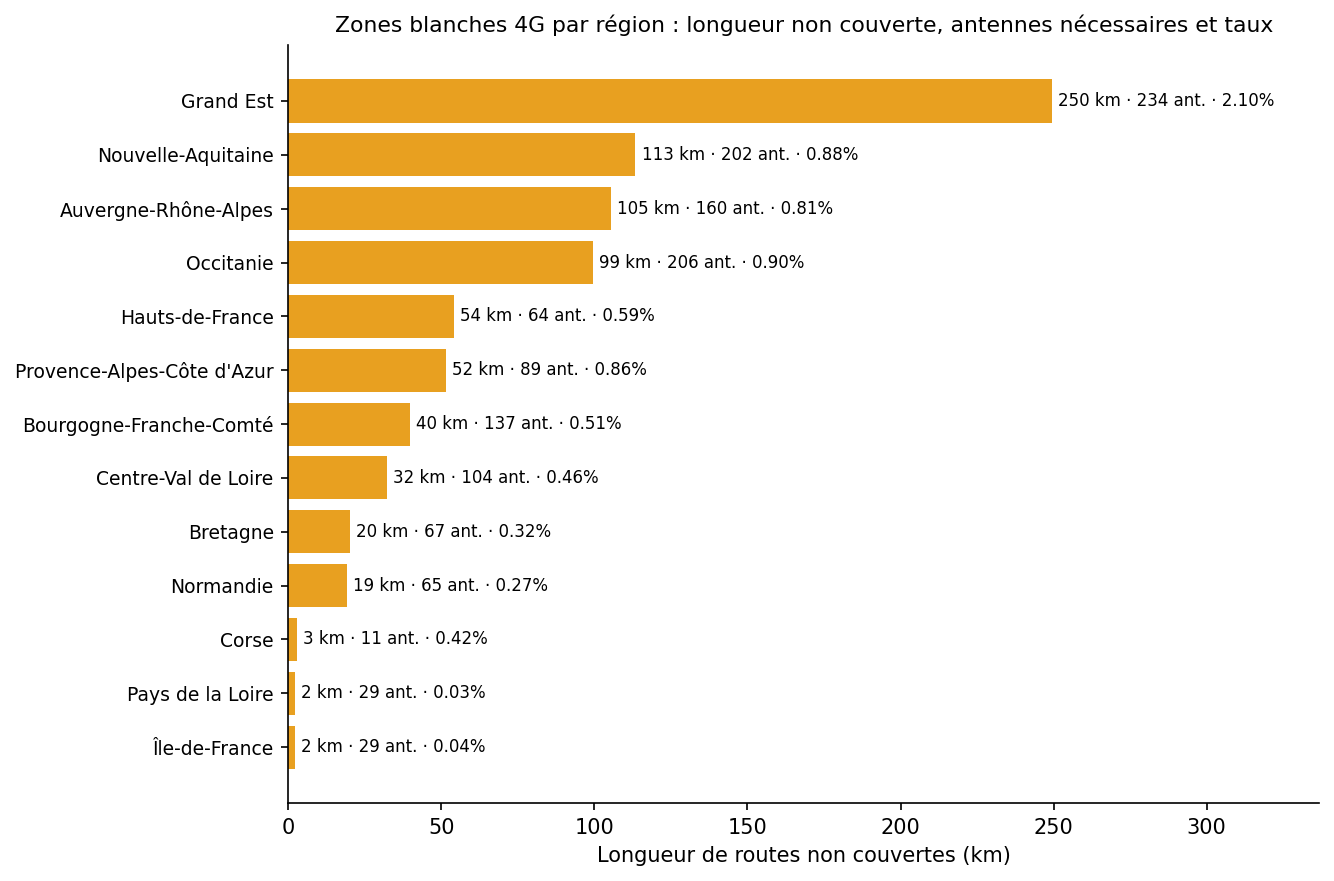
\includegraphics[width=\linewidth]{figures/regions_barres.png}
  \caption{Longueur de routes non couvertes par région, annotée du nombre d'antennes nécessaires et du taux de non-couverture. Le Grand Est concentre à lui seul près d'un tiers des zones blanches du réseau structurant.}
  \label{fig:regions}
\end{figure}

À l'échelle départementale, la dispersion est forte (table~\ref{tab:depts}). La Lozère présente le \emph{taux} de non-couverture le plus élevé (10{,}06~\%), conséquence d'un réseau structurant peu dense traversant un relief marqué. En \emph{volume}, le Haut-Rhin (86{,}9~km), les Pyrénées-Atlantiques (78{,}1~km) et la Moselle (67{,}2~km) dominent, traduisant des linéaires de montagne (Vosges, Pyrénées) ou frontaliers.

\begin{table}[H]
  \centering
  \caption{Dix départements au plus fort taux de non-couverture.}
  \label{tab:depts}
  \small
  \begin{tabular}{llrrr}
    \toprule
    \textbf{Dépt.} & \textbf{Région} & \textbf{Long. NC (km)} & \textbf{\% non couv.} & \textbf{Seg. NC} \\
    \midrule
    Lozère (48)                  & Occitanie                  & 37{,}5 & 10{,}06 & 132 \\
    Haut-Rhin (68)               & Grand Est                  & 86{,}9 & 8{,}92  & 233 \\
    Pyrénées-Atlantiques (64)    & Nouvelle-Aquitaine         & 78{,}1 & 6{,}82  & 226 \\
    Ardennes (08)                & Grand Est                  & 47{,}8 & 5{,}56  & 120 \\
    Territoire de Belfort (90)   & Bourgogne-Franche-Comté    & 8{,}5  & 4{,}72  & 43  \\
    Moselle (57)                 & Grand Est                  & 67{,}2 & 3{,}80  & 317 \\
    Savoie (73)                  & Auvergne-Rhône-Alpes       & 34{,}7 & 3{,}17  & 47  \\
    Ain (01)                     & Auvergne-Rhône-Alpes       & 33{,}7 & 2{,}46  & 410 \\
    Pyrénées-Orientales (66)     & Occitanie                  & 20{,}4 & 2{,}23  & 119 \\
    Alpes-de-Haute-Provence (04) & Provence-Alpes-Côte d'Azur & 13{,}8 & 2{,}06  & 32  \\
    \bottomrule
  \end{tabular}
\end{table}

\subsection{Préconisation : implantation de nouvelles antennes}

L'algorithme glouton de couverture d'ensemble (étape~3) estime qu'il faudrait \textbf{1\,397 nouvelles antennes} (rayon~1\,500~m) pour résorber l'intégralité des 4\,456~portions non couvertes. La figure~\ref{fig:antennes} en cartographie l'implantation, qui épouse logiquement la géographie des zones blanches : axes de montagne, littoraux et secteurs ruraux peu denses.

Le nombre d'antennes par territoire ne suit pas strictement la longueur non couverte, mais bien la \emph{fragmentation} des zones blanches. Ainsi le Grand Est, où les zones blanches sont à la fois nombreuses et étendues, requiert le plus d'antennes (234). À l'inverse, l'Aveyron arrive en tête des départements (45~antennes) pour seulement 10~km non couverts : ses zones blanches sont éparpillées en une multitude de courts tronçons, chacun exigeant sa propre antenne, alors qu'un département comme le Haut-Rhin résorbe un linéaire plus long avec proportionnellement moins d'antennes grâce à des segments plus contigus. Cette préconisation constitue une borne haute : elle ignore la portée réelle variable des antennes selon le relief et la possibilité de mutualiser une implantation avec les pylônes existants.

\begin{figure}[H]
  \centering
  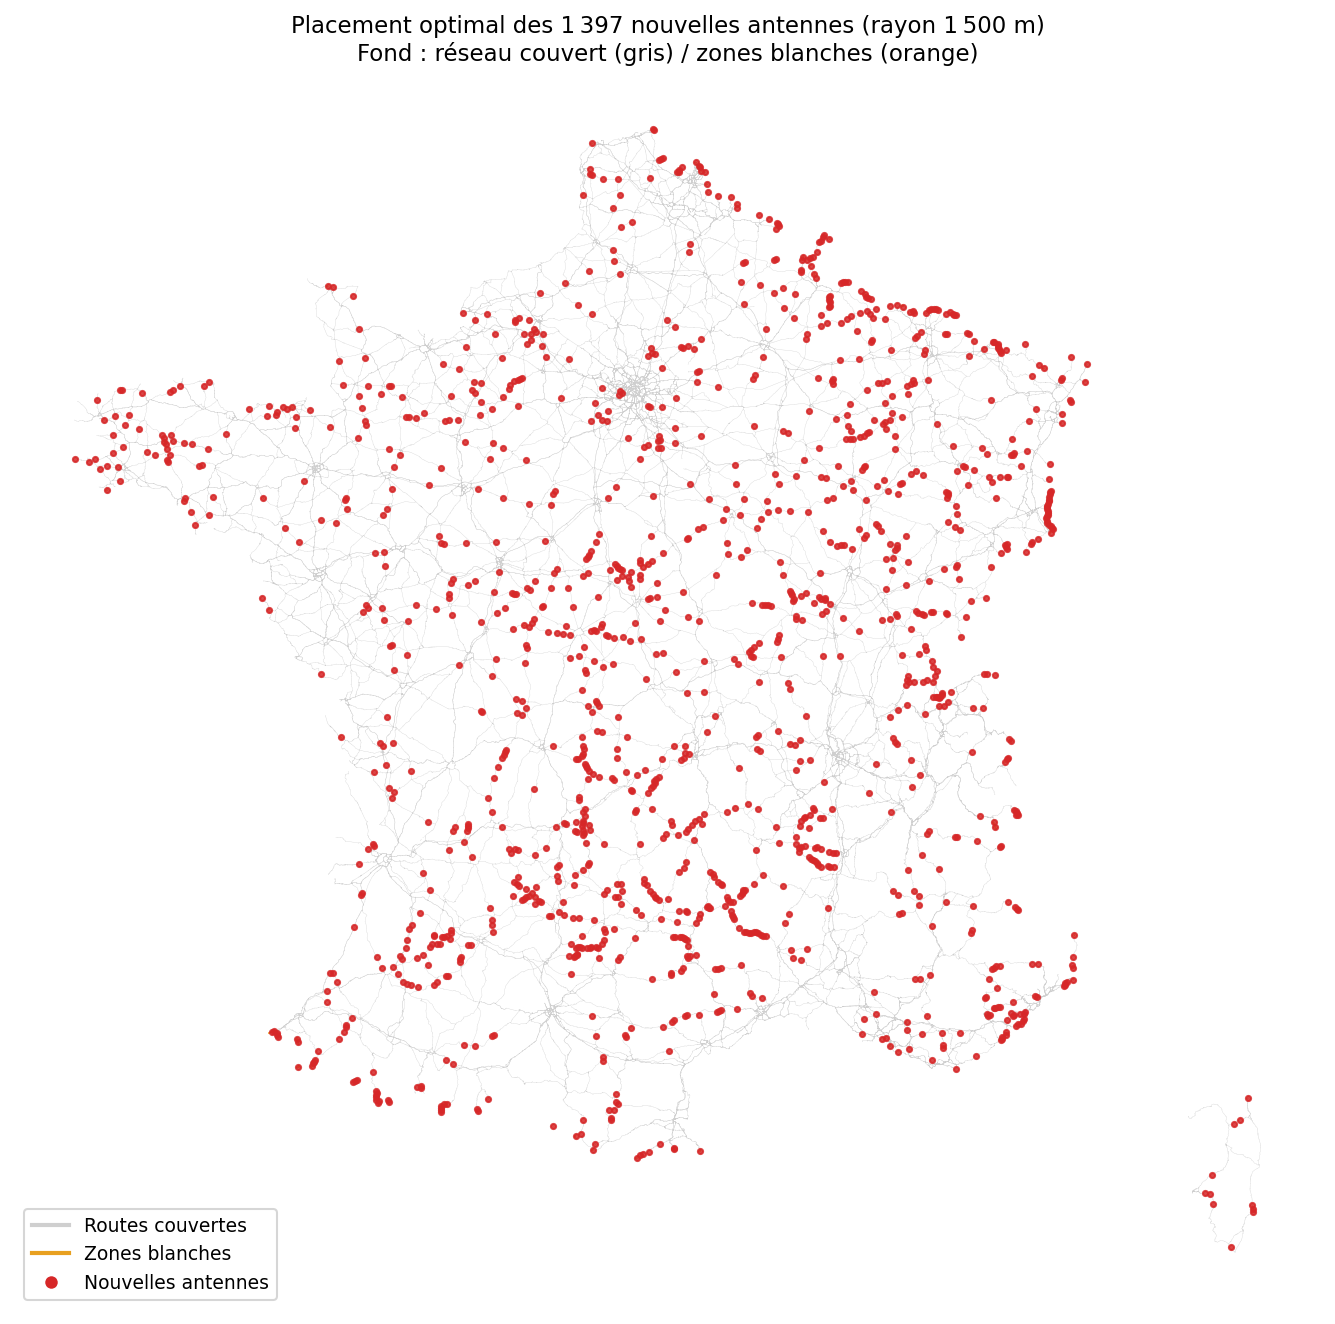
\includegraphics[width=0.82\linewidth]{figures/carte_antennes.png}
  \caption{Implantation des 1\,397 nouvelles antennes (points rouges) proposées par le \emph{greedy Set Cover}, sur fond de réseau couvert (gris) et de zones blanches (orange). La forme du territoire est dessinée par le seul réseau routier structurant.}
  \label{fig:antennes}
\end{figure}

% ============================================================
\section{Choix techniques et difficultés}\label{sec:perfs}
% ============================================================

\subsection{De l'overlay global à l'overlay tuilé}

La première version de l'étape~2 reposait sur la chaîne classique de GeoPandas : construction d'un \texttt{MultiPolygon} global de couverture (\emph{dissolve}), puis \texttt{gpd.overlay} en \emph{intersection} et en \emph{difference} contre l'ensemble des routes. Lancée en arrière-plan via \texttt{nohup}, elle a révélé des durées prohibitives (table~\ref{tab:perfs}).

\begin{table}[H]
  \centering
  \caption{Temps d'exécution observés sur la \emph{première} version de l'étape~2 (overlay global, abandonnée).}
  \label{tab:perfs}
  \begin{tabular}{lr}
    \toprule
    \textbf{Phase} & \textbf{Durée} \\
    \midrule
    Lecture des routes                          & $\sim$2 min \\
    Lecture de la couverture                    & $\sim$2{,}5 min \\
    Réparation des géométries                   & $\sim$33 min \\
    Dissolve de la couverture                   & $\sim$5 h 44 min \\
    Simplification de l'union                   & $\sim$5 min \\
    Overlay \emph{intersection} (routes couvertes)     & $\sim$10 jours \\
    Overlay \emph{difference} (routes non couvertes)   & $\sim$8 jours \\
    Écriture des sorties                        & $\sim$1{,}5 min \\
    \midrule
    \textbf{Total}                              & $\sim$20 jours \\
    \bottomrule
  \end{tabular}
\end{table}

Les deux overlays constituaient de loin le goulot d'étranglement. Cela tient à la nature de l'opération : pour chaque segment de route, GEOS doit calculer une intersection géométrique exacte avec un \texttt{MultiPolygon} extrêmement complexe (la couverture fusionnée, faite de plusieurs millions de sommets). Même avec un index spatial, le coût par segment reste élevé, et l'opération s'exécute sur un seul cœur.

\paragraph{Refonte tuilée et multithreadée.}
La version finale de \texttt{routes\_couvertes.py} (décrite plus haut, méthodologie étape~2) lève ce verrou par trois leviers complémentaires :
\begin{itemize}
  \item \textbf{Suppression de l'union globale.} Aucune couverture globale n'est plus construite : chaque tuile ne réalise qu'une \emph{union locale} des polygones qui la touchent, comportant infiniment moins de sommets. Le coût d'intersection par segment s'effondre.
  \item \textbf{Tuilage spatial.} La grille $8\times8$ borne le travail à des sous-problèmes indépendants et géographiquement compacts, où l'index \texttt{STRtree} élague l'essentiel des candidats.
  \item \textbf{Parallélisme réel.} Shapely~2 relâchant le GIL pendant les appels GEOS, les 64~tuiles (comme la réparation des géométries) sont traitées en parallèle sur tous les cœurs via un \texttt{ThreadPoolExecutor}, sans la surcharge mémoire d'un multiprocessing.
\end{itemize}
Ces optimisations — précisément les pistes que la première version reléguait aux perspectives — ramènent le croisement de \emph{plusieurs semaines} à une \emph{exécution unique}, soit un gain de un à deux ordres de grandeur. La durée exacte dépend du nombre de cœurs de la machine et n'a pas fait l'objet d'un \emph{benchmark} formel sur la version finale, mais le calcul, autrefois étalé sur près de trois semaines, tient désormais en une seule session de traitement.

\subsection{Difficultés rencontrées}

\paragraph{Volumétrie mémoire en étape 1.} La première version du script de fusion chargeait les quatre opérateurs en mémoire avant l'union finale, ce qui dépassait les capacités de notre machine. La version finale dissout chaque opérateur séparément et n'agrège que les quatre géométries simplifiées en mémoire au moment de l'union finale.

\paragraph{Géométries invalides.} Les exports ARCEP contiennent un nombre non négligeable de polygones invalides (auto-intersections, anneaux dégénérés). Sans correction, Shapely lève des exceptions \texttt{TopologyException} en cascade. Notre stratégie — \texttt{shapely.buffer(arr, 0)} vectorisé, repli sur \texttt{make\_valid()} pour les géométries restant invalides ou vides, puis filtrage des résultats non polygonaux — a permis de tout traiter sans perte significative, et son application par blocs parallèles a rendu cette passe négligeable dans le temps total.

\paragraph{CRS mal taggé.} Comme évoqué en méthodologie, le GeoPackage de couverture fusionnée pouvait être lu avec un CRS générique \texttt{Undefined geographic SRS} (voire absent), malgré des coordonnées clairement projetées. L'heuristique \texttt{looks\_like\_lonlat()} corrige ce cas par un \emph{override} EPSG:2154 sans reprojection.

\paragraph{Partage thread-safe de l'index spatial.} Le passage au multithreading impose de ne partager entre threads que des structures en lecture seule. L'index \texttt{STRtree} de la couverture est donc construit une seule fois dans le thread principal, puis interrogé (\texttt{query}, \texttt{dwithin}) sans modification par les workers ; les écritures se limitent à des sous-tableaux \texttt{numpy} disjoints, évitant tout verrou.

\paragraph{Choix de la tolérance de simplification.} La première version simplifiait l'\emph{union globale} à 50~m. La version tuilée simplifie au contraire chaque \emph{union locale} à 200~m : appliquée à l'échelle d'une tuile et uniquement pour accélérer l'overlay (et non pour le rendu cartographique), une tolérance plus grossière reste sans effet visible sur les longueurs calculées tout en réduisant nettement le nombre de sommets manipulés par GEOS.

% ============================================================
\section{Conclusion et perspectives}
% ============================================================

\subsection{Synthèse}

Le projet a abouti à une cartographie nationale des zones blanches 4G sur le réseau des grands axes, avec un taux de couverture cumulée des quatre opérateurs de \textbf{99{,}26~\%}, soit environ \textbf{792~km} de routes principales non couvertes. Le pipeline développé est entièrement reproductible : il prend en entrée les GeoPackages ARCEP bruts et une extraction OSM, et produit en sortie deux couches géographiques (routes couvertes, routes non couvertes), des statistiques par département et par région, ainsi qu'une préconisation d'implantation de \textbf{1\,397} nouvelles antennes pour résorber l'ensemble des zones blanches.

Sur le plan technique, le projet a mis en évidence l'importance des stratégies d'optimisation lorsqu'on travaille sur de très grands jeux de données géographiques. La refonte de l'étape de croisement — passage d'un \emph{overlay} global de plusieurs semaines à un \emph{overlay} tuilé et multithreadé s'exécutant en une seule session — illustre à elle seule le gain qu'apportent le tuilage spatial, l'union locale, l'indexation \texttt{STRtree} et le parallélisme réel permis par la libération du GIL dans GEOS, en complément de la gestion défensive des métadonnées CRS et des opérations vectorisées.

\subsection{Limites}

\begin{itemize}
  \item \textbf{Couvertures théoriques} : les données ARCEP sont issues de simulations de propagation, et non de mesures terrain. La couverture réelle peut différer.
  \item \textbf{4G uniquement} : la 5G et la 3G n'ont pas été intégrées. Un usager dont le terminal bascule en 3G en zone 4G blanche peut percevoir la couverture comme satisfaisante.
  \item \textbf{Définition permissive} : un segment est considéré couvert dès qu'un seul des quatre opérateurs le couvre, ce qui surestime la couverture du point de vue d'un usager fidèle à un seul opérateur.
  \item \textbf{Simplification 200~m} : la simplification locale appliquée par tuile accélère l'overlay mais rend les contours couvert/non couvert non exacts au mètre près à grande échelle (zoom local).
  \item \textbf{Modèle d'antennes simplifié} : le \emph{Set Cover} suppose un rayon de couverture uniforme de 1\,500~m et ignore le relief, la portée réelle variable des antennes et les pylônes existants mutualisables. Le chiffre de 1\,397~antennes constitue donc une borne haute indicative, non un plan de déploiement.
\end{itemize}

\subsection{Perspectives}

Le tuilage spatial parallèle, envisagé comme perspective dans une version antérieure de ce rapport, a été implémenté et constitue désormais le cœur de l'étape~2. Plusieurs autres extensions restent envisageables :
\begin{itemize}
  \item \textbf{Analyse par opérateur} : conserver les quatre couvertures séparées pour produire un score de couverture par segment (de 0 à 4 opérateurs).
  \item \textbf{Raffinement du placement d'antennes} : remplacer le rayon fixe par une portée dépendant du relief, intégrer les pylônes existants comme sites candidats prioritaires et pondérer par un coût d'implantation, pour passer d'une borne haute à un véritable scénario de déploiement.
  \item \textbf{Croisement démographique} : intersecter les zones blanches avec la grille de population INSEE pour évaluer combien d'habitants traversent quotidiennement une zone blanche.
  \item \textbf{Comparaison temporelle} : reproduire l'analyse sur plusieurs trimestres successifs pour mesurer l'évolution de la couverture.
  \item \textbf{Extension à la 5G} : intégrer les couches 5G ARCEP, désormais disponibles pour les quatre opérateurs.
\end{itemize}

% ============================================================
\appendix
\section*{Annexe : reproduction des résultats}
\addcontentsline{toc}{section}{Annexe : reproduction des résultats}

Le pipeline est organisé en trois scripts Python autonomes :
\begin{itemize}
  \item \textbf{\texttt{merge\_coverage\_optimized.py}} (étape 1) : prend en entrée les quatre GeoPackages opérateurs ARCEP, applique réparation, simplification (50~m) et \emph{dissolve} par opérateur avec checkpoints intermédiaires, puis produit la couverture fusionnée \texttt{couverture\_4G\_totale.gpkg} (réutilisée comme \texttt{coverage\_4G\_france.gpkg} en entrée de l'étape~2). Durée estimée : environ 6~heures.
  \item \textbf{\texttt{routes\_couvertes.py}} (étape 2) : prend en entrée la couverture fusionnée et l'extraction OSM des grands axes (\texttt{grand\_axe\_2154.gpkg}), et produit \texttt{routes\_couvertes.gpkg} et \texttt{routes\_non\_couvertes.gpkg} via l'overlay tuilé multithreadé. Durée : une seule session de traitement (contre $\sim$20~jours pour la version initiale non tuilée). Paramètres principaux : grille $8\times8$, tolérance de simplification locale 200~m, nombre de threads égal au nombre de cœurs.
  \item \textbf{\texttt{analyse\_zones\_blanches.py}} (étape 3) : prend en entrée les deux couches précédentes, télécharge les contours administratifs IGN (cache \texttt{admin\_france.gpkg}), et produit \texttt{stats\_departements.csv}, \texttt{stats\_regions.csv}, \texttt{rapport\_antennes.csv} et \texttt{nouvelles\_antennes.gpkg}. Paramètre principal : rayon d'antenne 1\,500~m. Un accès réseau à la Géoplateforme est requis au premier lancement (ou un \texttt{admin\_france.gpkg} fourni manuellement).
\end{itemize}

Les prérequis sont Python 3.9+ avec les bibliothèques \texttt{geopandas}, \texttt{shapely} (version $\geq$ 2.0), \texttt{pyogrio}, \texttt{numpy} et \texttt{pandas}.

\end{document}